\chapter{QUADRO TEÓRICO}

\par Neste capítulo serão listados os conceitos e as tecnologias que serão
utilizados no desenvolvimento da proposta de trabalho apontada na seção 
objetivos. Para tal, serão discutidos a definição, o histórico e as 
aplicabilidades de cada um deles, tomando por base autores fundantes e 
seus comentaristas. É importante ressaltar que o texto desta sessão, quando
descreve a teoria da evolução das espécies, não tem como objetivo levantar
questões sobre a origem dos seres vivos.

\section{Algoritmos Genéticos}

\subsection{Fundamentos}

\par Para \citeonline{livro_introduction_ag_melaine_mitchell}, desde o começo da
era computacional, cientistas pioneiros, tais como Alan Turing, John von
Neumann, Norbert Wiener e outros, tinham o objetivo de dotar os computadores de inteligência
de maneira que eles pudessem tomar decisões, se adaptar a determinadas situações
e até mesmo ter a capacidade de aprender. Com esta motivação, estes cientistas
se interessaram por outras áreas, além da eletrônica, como  a
biologia e a psicologia e começaram então a realizar pesquisas para simular os
sistemas naturais no mundo computacional a fim de alcançarem suas metas. 

\par Vários conceitos computacionais baseados na natureza surgiram então ao
longo do tempo, dentre eles a computação evolucionária inspirada na teoria da evolução natural
a qual o exemplo mais proeminente são os AGs que foram introduzidos por Jhon Holland, seu aluno
David Goldberg e outros estudantes da universidade de Michigan.
\citeonline{livro_genetic_algorithm_goldberg} define os AGs como métodos de busca baseados na
genética e no mecanismo de seleção natural que permitem a possibilidade de obter
robustez e eficácia na tarefa de encontrar uma solução boa para um problema em um espaço de busca
complexo em um tempo aceitável.


\par A teoria da evolução foi proposta pelo naturalista inglês Charles
Darwin por volta de 1850, quando este, em uma viagem de navio visitou vários lugares e, 
por ser uma pessoa com uma grande habilidade de  observação, percebeu que
indivíduos de uma mesma espécie vivendo em lugares diferentes possuíam também
características distintas, ou seja, cada indivíduo  possuía atributos
específicos que lhe permitia uma melhor adaptação em seu ecossistema. 


\par Com base nesta observação, Darwin então propôs que existe um processo de
seleção natural, afirmando que, como os recursos na natureza, tais como água e comida,
são limitados, os indivíduos competem entre si e aqueles que não possuem atributos necessários
à adaptação ao seu ambiente tendem a ter uma probabilidade menor de reprodução e
irão ser extintos ao longo do tempo, e por outro lado, aqueles
com características que os permitem obter vantagens competitivas no meio onde
vivem acabam tendo mais chances de sobreviver e gerar indivíduos ainda mais
adaptados. 

\par A teoria ressalta porém que, o processo não tem o objetivo de maximizar
algumas características das espécies, pois  os novos indivíduos
possuem atributos que são resultados da mesclagem das características dos reprodutores,
o que faz com que os filhos não sejam exatamente iguais aos pais, podendo assim
ser superiores, uma vez que, estes herdem as qualidades de seus pais ou
inferiores se os descendentes herdarem as partes ruins de seus
reprodutores. Este processo de transferência de informação será explicado
posteriormente \cite{livro_ags_ricardo_linden}.

\par Para entender a relação entre AGs e a evolução natural é
necessário conhecer as principais terminologias biológicas, 
sendo importante ressaltar porém que, de acordo com
\citeonline{livro_introduction_ag_melaine_mitchell}, apesar da 
analogia a certos termos da biologia, a forma com que os AGs 
são implementados é relativamente simples se comparado ao funcionamento
biológico real.

\par \citeonline{livro_introduction_ag_melaine_mitchell} afirma que 
todos os seres vivos são compostos de células e estas possuem um ou mais
cromossomos que, basicamente, são manuais de instruções que definem as 
características do organismo. O cromossomo é formado por um conjunto de genes
que, em grupo ou individualmente, são responsáveis por um determinado atributo
do indivíduo como por exemplo, a cor do cabelo, a altura e etc. Cada gene possui
uma localização dentro do cromossomo denominada locus e, por fim, o conjunto de
todos os cromossomos dentro da célula é definido como genoma. 

\par Considerando isto, \citeonline[p.33]{livro_ags_ricardo_linden} afirma que,

\begin{citacao}
Um conjunto específico de genes no genoma é chamado de genótipo. O
genótipo é a base do fenótipo, que é a expressão das características
físicas e mentais codificadas pelos genes e modificadas pelo
ambiente, tais como cor dos olhos, inteligência etc. Daí, podemos concluir: nosso
DNA codifica toda a informação necessária para nos descrever, mas esta
informação está sob controle de uma grande rede de regulação gênica
que, associada às condições ambientais, gera as proteínas na quantidade
certa, que farão de nós tudo aquilo que efetivamente
somos.
\end{citacao}  

\par Uma vez descrita a complexidade dos organismos é necessário discorrer,
de forma básica, sobre o processo de reprodução responsável pela
transmissão da informação genética de geração para geração.

\par Existem dois tipos de reprodução, a assexuada, em que não é necessário a
presença de um parceiro e a sexuada que exige a presença de dois organismos.
Os AGs simulam a reprodução sexuada em que cada um dos organismos envolvidos
oferece um material genético denominado gametas. As gametas são formadas através de
um processo denominado \textit{crossing-over} ou \textit{crossover} que tem
início com a divisão de cada cromossomo em duas parte as quais 
irão se cruzar uma com a outra para formar dois novos cromossomos, que
receberão um pedaço de cada uma das partes envolvidas no cruzamento.

\par O resultado deste processo será então quatro cromossomos potencialmente
diferentes que irão compor as gametas e farão parte do novo indivíduo. Neste processo
pode ocorrer mutações que são resultados de alguns erros ou da influência
de algum fator externo, como a radiação por exemplo. Estas mutações são
pequenas mudanças nos genes do indivíduos, podendo estas ser boas, ruins ou neutras.


\par E assim a informação genética é passada dos pais para os filhos, e como os
componentes dos cromossomos definem as características do organismo, os filhos
herdarão características dos pais porém serão ligeiramente diferente deles, como
foi descrito anteriormente, o que permite que os novos indivíduos herdem
características melhores ou piores que seus progenitores, porém, se os pais
possuem características positivas, a probabilidade de gerarem filhos ainda
melhores são maiores \cite{livro_ags_ricardo_linden}.

\subsubsection{Características dos Algoritmos Genéticos}

\par De acordo com \citeonline{livro_ags_ricardo_linden}, a analogia dos AGs com
os processos biológicos se dá por meio da representação de cada termo descrito
anteriormente em um modelo computacional voltado a encontrar soluções a um
determinado problema em um processo aleatório. O fluxo de execução deste processo
inicia-se com a criação aleatória de uma população inicial. Uma população contém
um conjunto de indivíduos sendo que cada indivíduo  representa uma possível solução
para o problema.

\par O autor afirma ainda que, um indivíduo é formado por cromossomos que
guardam as características da solução, ou seja, a forma que esta resolve o
problema.

\subsubsection{Função de avaliação}

\par Segundo \citeonline{livro_ags_ricardo_linden} após a criação da população
inicial esta é então avaliada através de uma função de avaliação que mede a qualidade de cada uma de suas soluções e é
realizado então uma classificação que ordena as soluções das melhores para as
piores, para então iniciar a formação de uma nova população. A nova população
pode conter já inicialmente os dois melhores indivíduos existentes, este
mecanismo é denominado elitismo e pode ser utilizado ou não.

\par Ainda segundo o autor a função de Avaliação ou função de aptdão penaliza as
soluções inviáveis para a solução do problema,ou seja, ao verificar que uma
certa solução não satisfaz o grau de aptidão nescessário para o problema
proposto esta solução é descartada e assim, só sobrevivem na execução da função
as soluções com mais chence de resolver o problema e por isso torna-se o
componente mais importante de qualquer algoritmo genetico.

\par Devido a generilidade encontrada nos GAs a função de avaliação
torna-se em muitos casos a unica ligação verdadeira entre o programa e o problema real, por
isso deve-se ter um certo cuidado ao escolhe-la, ela deve conter tudo o que se
sabe sobre o problema a ser resolvido, quanto mais conhecimento a função
possuir, maior será a chance da função entregar o melhor resultado
\cite{livro_ags_ricardo_linden}.

% \par Baseando nessas \citeonline{livro_ags_ricardo_linden}, iremos
% usar no projeto uma função para avaliar dentre varias costureiras a melhor forma de
% destribuir a materia prima para que seja produzida uma certa quantidade de
% calças no menor tempo possível.


\subsubsection{Seleção}

\par Segundo \citeonline{livro_ags_ricardo_linden}, o próximo passo
para a formação da nova população é o cruzamento que, inicia-se com a seleção de
dois indivíduos, que é realizada de acordo com a qualidade destes, porém,
como é fundamental que esta escolha não despreze completamente os indivíduos com uma
qualidade muito baixa, a seleção é feita de forma probabilística ou seja
indivíduos com boa qualidade possuem mais chances de serem selecionados e, por outro lado,
indivíduos com menor nota de avaliação terão menos chance.

\par Para \citeonline{livro_ags_ricardo_linden}, é importante que não se tenha
apenas as melhores soluções, as soluções com menor grau de avalição também são
importantes para que se tenha uma maior diversidade de caracteristicas na
população envolvida para solução do problema, possibilitanto uma maior evolução
da população para proseguir de forma satisfatória, pois se esta for
constituida somente das melhores soluções, será composta de indídudos
cada vez mais semelhantes prejudicando a evolução da população.


Existe vários tipos, mas iremos usar a X por causa disso

\subsubsection{Cruzamento}
\par Após a seleção dos pais irá ocorrer então o processo de \textit{crossover}
e, como no cruzamento natural, neste processo dois novos indivíduos, ou seja, duas
novas soluções são formadas a partir de características daquelas que se
cruzaram, ou seja, serão geradas duas novas soluções que conterão alguns cromossomos
de uma solução e alguns cromossomos de outra.

Existe vários tipos, mas iremos usar a X por causa disso

\subsubsection{Mutação}

\par Para o autor, também pode ocorrer a mutação em
que, da mesma forma que ocorre na natureza, aleatoriamente o valor dos
cromossomos de um indivíduo pode ser alterado. A mutação ocorre de acordo com
uma taxa definida. Basicamente é definido uma porcentagem baixa e então um
número de 0 a 1 é sorteado e multiplicado por 100, se o resultado for menor que
a porcentagem então irá ocorrer a mutação para aquele indivíduo.

Existe vários tipos, mas iremos usar a X por causa disso

\par Concluindo, \citeonline{livro_ags_ricardo_linden} afirma que o processo de 
seleção, cruzamento e mutação acontece até formar uma nova população, 
quando isto acontece todos os indivíduos da população anterior são
desconsiderados e então a nova população é submetida a todo o processo
novamente, passando pela avaliação, classificação, cruzamento, mutação para
formar assim uma nova população. O fim da execução acontece quando o
número de populações criadas atinge um limite que é definido previamente.
Este processo oferece como saída a melhor solução encontrada.


\subsubsection{Como Funciona}

\par Para entendermos como os AGs funcionam temos que saber alguns passsos
fundamentais para desenvolver uma solução usando AGs e esses passos são:
\item Inicialize a população de cromossomos;
\item Avalie cada cromossomo na população;
\item Selecione os pais para gerar novos cromossomos;
\item Aplique os opreradores de recombinação e mutação a estes pais de forma a
gerar os indivíduos da nova geração;
\item Apague os velhos membros da população;
\item Avalie todos os novos cromossomos e insira-os na população
\item Se o tempo acabou o melhor cromossomo satisfaz os requerimentos e
desempenho, retorne-o, caso contrario, selecione os pais para gerar novos
cromossomos

\par Estes passos são o básico para que se possoa desenvolver uma solução
utilizando AGs e escondem uma complexibilidade do processo de obtenção de alguns
elementos como:
\item uma melhor forma de criar os cromossomos para se adequar na resolução do
problema;
\item uma função de avaliação para que dentre vairias soluções
sempre seja mantida a melhor solução para que se possa chegar ao resultado
esperado ou bem próximo do esperado de um problema e descarte as soluções que
não estão aptas a serem usadas para atingir a solução do problema;

\section{Orientação a Objetos}

\par Para \citeonline{livro_intro_a_prog_orientada_objetos_usando_java},
programação orientada a objetos é um paradigma de programação que usa
classes e objetos, criados a partir de modelos, para representar e processar
dados usando aplicações em computadores.

\par Os modelos são simplificações do mundo real, que representam
objetos, pessoas, itens, tarefas, ideias, etc. usados comumente por
pessoas no dia a dia, independente do uso de computadores. 
Os dados pertencentes aos modelos são representados por tipos nativos,
característicos das linguagem de programação e podem também ser representados
por modelos criados pelo
programador \cite{livro_intro_a_prog_orientada_objetos_usando_java}.

\par \citeonline{livro_intro_a_prog_orientada_objetos_usando_java}
exemplifica um modelo como por exemplo para representar uma pessoa empregada de
uma empresa para fins de processamento de folha de pagamento, neste caso o
modelo representaria dentre outros dados, o nome, cargo, salário e horas extras
trabalhadas dessa pessoa, ainda podendo conter operações para realização
de cálculos de salário por exemplo.


\par Concluindo, \citeonline{ifsudestemg} afirma que, do mesmo modo 
que no mundo real vemos as coisas de um ângulo geral em que objetos se
interagem entre si, a proposta de orientação a objetos é que uma  
aplicação não seja organizada em processos estruturados mas
sim como objetos que se interagem uns com os outros.

\subsubsection{Como Funciona}

\par Para entendermos como os AGs funcionam temos que saber alguns passsos
fundamentais para desenvolver uma solução usando AGs e esses passos são:
\item Inicialize a população de cromossomos;
\item Avalie cada cromossomo na população;
\item Selecione os pais para gerar novos cromossomos;
\item Aplique os opreradores de recombinação e mutação a estes pais de forma a
gerar os indivíduos da nova geração;
\item Apague os velhos membros da população;
\item Avalie todos os novos cromossomos e insira-os na população
\item Se o tempo acabou o melhor cromossomo satisfaz os requerimentos e
desempenho, retorne-o, caso contrario, selecione os pais para gerar novos
cromossomos

\par Estes passos são o básico para que se possoa desenvolver uma solução
utilizando AGs e escondem uma complexibilidade do processo de obtenção de alguns
elementos como:
\item uma melhor forma de criar os cromossomos para se adequar na resolução do
problema;
\item uma função de avaliação para que dentre vairias soluções
sempre seja mantida a melhor solução para que se possa chegar ao resultado
esperado ou bem próximo do esperado de um problema e descarte as soluções que
não estão aptas a serem usadas para atingir a solução do problema;
\item 



% \par Para \citeonline[p.4]{ifsudestemg}, a proposta da Orientação a
% Objetos é,
% 
% \begin{citacao}
% Representar o mais fielmente possível as
% situações do mundo real nos sistemas computacionais. Nós entendemos o mundo
% como um todo composto por vários objetos que interagem uns com os outros. Da
% mesma maneira, a Orientação a Objetos consiste em considerar os sistemas
% computacionais não como uma coleção estruturada de processos, mas sim como
% uma coleção de objetos que interagem entre si.
% \end{citacao}  


% 
% Este processo é iniciado com um conjunto de várias soluções
% candidatas que fazem alusão aos cromossomos e cada solução possui atributos que
% definem como o problema pode ser resolvido. Tais atributos fazem alusão aos
% genes e os valores que estes atributos podem assumir, seja um valor numérico,
% ou um texto, por exemplo, fazem referência aos alelos. Após estas definições 
% durante a execução do algoritmo, ocorre o processo de reprodução em que as
% soluções se cruzam entre si, simulando o processo de \textit{crossing-over} no
% intuito de gerarem soluções possivelmente melhores, alem disto também é simulado
% o processo de mutação em que aleatóriamente um atributo de uma solução pode ser alterado.
% No final deste processo existe um mecanismo que mede a qualidade das soluções
% geradas e o processo continua até que a melhor solução seja encontrada ou até que o número
% de reproduções, definido préviamente, seja atingido, neste caso a melhor solução
% encontrada até aquele momento será o resultado do processo, ou seja, a melhor
% solução naquela execução, sendo importante ressaltar porém que outras execuções
% podem gerar resultados diferentes. \cite{livro_introduction_ag_melaine_mitchell}


\section{Tecnologias}

\par Abaixo serão listadas as tecnologias que serão utilizadas no
desenvolvimento do projeto.

\subsection{Java}

\par Segundo \citeonline{oracle}, a Linguagem Java foi projetada
para permitir o desenvolvimento de aplicações seguras, portáteis
e de alto desempenho para a mais ampla gama de plataformas de computação.

\par De acordo com \citeonline{livro_java_complete_references}, o Java foi
criado em 1991 pela \textit{Sun Microsystems} e foi baseado em uma linguagem já
existente, o C++, que foi escolhida por ser orientada a objetos e
por gerar códigos pequenos, o que era exatamente o que eles precisavam para
implantar em pequenos aparelhos. Além dessas características, um requisito
desejável era que a nova linguagem fosse independente de plataforma, para que
fosse executado em qualquer arquitetura, tais como, TVs, telefones, entre
outros, e então, para atender esta exigência, foi
criado o conceito de máquina virtual, que ficou conhecido como \textit{Java
Virtual Machine} - JVM\footnotemark[2].

\footnotetext[3]{O termo Java Virtual Machine será referenciado pela sigla JVM a
partir deste ponto do trabalho.}

\par O ponto chave que
permite o Java resolver o problema de portabilidade é o fato de o código ser
compilado em \textit{Bytecode} que é um conjunto genérico de instruções
altamente otimizado que é executado pela JVM, e esta, por sua vez, traduz o
mesmo para a arquitetura a qual ela está instalada o que possibilita a execução do programa
em várias plataformas \cite{livro_java_complete_references}.
%Ver este contexto resolvendo assim também problemas associados com programas baseados na web. 


% 
% \par Hoje os Browsers que possuem JVM embutida podem executar programas que 
% utilizam a linguagem JAVA. 
% 
% Neste particular Quinteiro (2006) registrou que:
% 
% \begin{citacao}
% “A Sun considera o sucesso do Java na Internet como sendo o primeiro passo para utilizá-lo em decodificadores da 
% televisão interativa, em dispositivos portáteis e outros produtos eletrônicos de consumo - exatamente como o Java 
% tinha começado em 1991. Sua natureza portátil e o projeto robusto permitem o desenvolvimento para múltiplas 
% plataformas, em ambientes tão exigentes como os da eletrônica de consumo".\cite[p.33]{livro_ags_ricardo_linden}
% \end{citacao}  


\par Além da portabilidade, o Java também é \textit{Multithread}, ou seja,
permite a execução de múltiplas tarefas, tem o \textit{automatic garbage
collector} que consiste em um mecanismo de gerenciamento de memória que a JVM
acomoda. Além disso o Java suporta uma extensa biblioteca de rotinas que
facilitam a interação com protocolos TCP/IP, como HTTP e FTP, além de possuir uma
segurança em sua execução por controlar programas via rede com
restrições \cite{livro_java_complete_references}.

\par De acordo com \citeonline{livro_java_Guia_do_Programador}, 

\begin{citacao} Atualmente a linguagem está organizada em três segmentos
principais:


	- JavaMe (\textit{Java Micro Edition})- Destinado a pequenos dispositivos
	computacionais móveis, tais como celulares, PDAs e set-top boxes. É composto de máquina virtuais otimizadas para ambientes mais restritos, especificações de 
funcionalidades e uma API mais compacta; 
	  
	- JavaSE (\textit{textJava Standard Edition})- Integra os elementos padrão
	da plataforma e permite o desenvolvimento de aplicações de pequeno e médio porte. Inclui todas as APIs consideradas de base,
além da máquina virtual padrão;

	- JavaEE (\textit{Java Enterprise Edition})- Voltada para o desenvolvimento
	de aplicações corporativas complexas. Adiciona APIs especificas aos elementos padrão da plataforma.
	

\end{citacao}

\subsection{AngularJS}

\subsubsection{Introdução}

\par Segundo \citeonline{livro_java_Guia_do_Programador} a lingugem Java Script
é uma das linguagens que vem sendo muito utilizada para desenvolver aplicações WEB. Com isso ela sempre esta em evolução e com isso
vão surgindo novos frameworks tornando-a cada dia mais poderosa e com mais
recursos e dentre esses frameworks está o AngularJS

\par O AngularJS é mantido pelo Google e possui varios recursos que o fazem uma
ferramenta poderosa.
Uma dessas particularidades é que ele funciona como uma extensão ao documento HTML, adici-
onando novos parâmetros e interagindo de forma dinâmica com vários elementos. Ou seja, com
AngularJS podemos adicionar novos atributos no html para conseguir adicionar funcionalidades
extras, sem a necessidade de programar em javascript.
AngularJS é quase uma linguagem declarativa, ou seja, você usa novos parâmetros na linguagem
html para alterar o comportamento padrão do html. Estes parâmetros (ou propriedades) são
chamados de diretivas.
Além disso, é fornecido também um conjunto de funcionalidades que tornam o desenvolvimento
web muito mais fácil, tais como o DataBinding, templates e fácil uso do Ajax
\cite{livro_java_Guia_do_Programador}.

\subsubsection{Características}

\par O AngularJS possui algumas caracteríticas e através delas será possível
realizar diferentes tarefas que irão tornar o desenvolvimento web muito mais simples e prazeroso.

\subsubsection{DataBind}

\par O DataBind é uma das principais vantagens do AngularJS.
Com ele conseguimos ligar automaticamente uma variável qualquer a uma outra.
Geralmente, é usado para ligar uma variável do JavaScript (ou um objeto) a algum
elemento do documento HTML \cite{livro_java_Guia_do_Programador}.

\subsubsection{Controller}

\par Um controller é um arquivo JavaScript que contém funcionalidades
referentes à alguma parte do documento HTML.
Não existe uma regra para o controller, como por exemplo
ter um controller por arquivo HTML, mas sim uma forma de sintetizar as regras de negócio (funções
javascript) em um lugar separado ao documento HTML
\cite{livro_java_Guia_do_Programador}.

\subsubsection{Loops}

\par Com o AngularJS pode-se utilizar templates para que se possa
adicionar conteúdo dinâmico. Um loop é sempre realizado através da propriedade ng-repeat e obedece a uma variável
que geralmente é um array de dados \cite{livro_java_Guia_do_Programador}.


% \subsection{Java Server Faces}
% 
% \par Segundo \citeonline{livro_programacao_java_para_web}, o \textit{JavaServer
% Faces} é uma especificação para um \textit{framework} de componentes para
% desenvolvimento \textit{web} em Java de forma segura. Foi definido pela
% \textit{Java Comunity Process} - JCP\footnotemark[3], que é uma entidade cujo
% objetivo é especificar a evolução do Java.
% 
% \footnotetext[4]{O termo \textit{Java Comunity Process} será referenciado pela
% sigla JCP a partir deste ponto do trabalho.}
% 
% \par Como o JSF é uma especificação da JCP, grandes empresas como
% \textit{Apache}, \textit{IBM}, \textit{Oracle} entre outras, participaram da
% definição do JSF e aprovaram sua especificação e mesmo sendo idealizado por várias empresas e generalizado pela
% JCP, o JSF torna-se um padrão de mercado, mas não é um produto acabado e precisa
% de implementações.\cite{livro_programacao_java_para_web}
% 
% \par As implementações mais conhecidas são:
% 
%  \begin{itemize}
% 	\item \textit{Sun Mojarra} (antes JSF R1) – implementação de referencia
% 	(http://javaserverfaces.java.net/)
% 	
% 	\item \textit{MyFaces} da \textit{Apache}(http://myfaces.apache.org/)
%  \end{itemize}
% 
% \par Com essa implementação é possível utilizar todos os recursos do padrão JSF,
% como formulários, tabelas, \textit{layout}, conversão e validação de eventos,
% além de toda a inteligência para a interpretação dos arquivos de configuração e
% interação com o contêiner Java. Como o JSF é um padrão de mercado, várias empresas investem no
% desenvolvimento de componentes como, Calendário, \textit{ProgressBar}, menus,
% efeitos de transição entre outros.\cite{livro_programacao_java_para_web}
% 
%  \par Algumas das principais bibliotecas de componentes são:
% 
%  \begin{itemize}
% 	\item \textit{Trinidad}, da \textit{Apache MyFaces}
% 	(http://myfaces.apache.org/trinidad/);
% 	
% 	\item \textit{Tobago}, da \textit{Apache MyFaces}
% 	(http://myfaces.apache.org/tobago/);
% 	
% 	\item \textit{ICEFaces}, da \textit{ICESoft} (http://www.icefaces.org/);
% 	
% 	\item \textit{RichFaces}, da \textit{JBoss} (http://www.jboss.org/richfaces/);
% 	
% 	\item \textit{Tomahawk}, da \textit{Apache MyFaces}
% 	(http://myfaces.apache.org/tomahawk/);
% 	
% 	\item \textit{PrimeFaces} (http://www.primefaces.org/)
%  \end{itemize}
% 
% \par Neste projeto, utilizaremos a biblioteca PrimeFaces.
% 



\subsection{Tomcat}

\par Segundo \citeonline{livro_apache_tomcat_7}, o \textit{Tomcat} é um
servidor \textit{open source} e \textit{container} de aplicativos \textit{web}
baseados em Java que foi criado para executar \textit{servlets} e \textit{JavaServer
Pages} - JSP\footnotemark[4].
Ele foi criado como um sub-projeto da \textit{Apache-Jakarta}, porém como ficou
muito popular entre os desenvolvedores, a \textit{Apache} o denominou como um
projeto separado e vem sendo melhorado e apoiado por um grupo de voluntários da comunidade \textit{Java Open
Source}, que o faz uma excelente solução para desenvolvimento de uma aplicação
\textit{web} completa. 
\footnotetext[5]{O termo JavaServer Pages será referenciado pela sigla JSP
a partir deste ponto do trabalho.}

% \par O \textit{Apache Tomcat} é um servidor web estável, ele 
% possui varias funcionalidades como o \textit{Tomcat Manager},
% \textit{Specialized Realm Implementations} e \textit{Tomcat Valves}. O
% \textit{Tomcat Manager} é fornecido com o servidor \textit{Tomcat} e é
% responsável pela funcionalidade básica para gerenciar aplicações web em execução no servidor \textit{Tomcat} 
% a partir de qualquer navegador. Ja o \textit{Specialized Realm Implementations}
% é um método de segurança que o Tomcat disponibiliza para proteger os recursos
% dentro do \textit{container} que é um recipiente que funciona como um banco de
% dados de usuários e esses bancos são denominados \textit{Realm}. O
% \textit{Tomcat Valves} é uma tecnologia que foi introduzido no Tomcat 4 e esta disponível nas versões
% posteriores e permitem associar instâncias de uma classe JAVA com um
% \textit{container} \textit{Catalina} particular, agindo como um pré-processador
% para todos os pedidos que vêm para o \textit{container}. 
% \cite{livro_apache_tomcat_7}



%\par Segundo a Apache (2015), o Tomcat é um software livre que realiza a
%implementação de especificações do Java voltado para programação para 
%internet lançado pela própria Apache.
% \par Exemplo de parágrafo utilizando comando para formatar em itálico as palavras em inglês, como por exemplo: \textit{pets, animals and software} e um exemplo de texto em negrigo: \textbf{grafo}.
% 
% \par Um tipo de citação: segundo \citeonline{correa2003plantas} as plantas \ldots.
% 
% \par Outro tipo de citação: as plantas \ldots \cite{correa2003plantas}.
% 
% \par Outro tipo de citação com página: \cite[p. 13]{correa2003plantas}.
% \par Outro tipo ainda de citação com página:  \citeonline[p. 13]{correa2003plantas}.
% 
% \par Para referenciar seções e capítulos, é necessário colocar o \textbackslash label e a referência assim: na \autoref{sec:materiais} e no \autoref{cap:quadroMetodologico} são encontradas as informações\ldots
% 
% \par Exemplo de equação:
% 
% \begin{equation}
%  \Delta Q = 
%  \left[
%  \frac{\sum_{in} + k_{i,in}}{2m} - 
%  \left(
%  \frac{\sum_{tot} + k_i}{2m}
%  \right)^2
%  \right] -
%  \left[
%  \frac{\sum_{in}}{2m} - 
%  \left(\frac{\sum_{tot}}{2m}
%  \right)^2 - 
%  \left(\frac{k_i}{2m}
%  \right)^2
%  \right]
% \end{equation}
% 
% 
% \par Símbolos matemáticos só funcionam dentro do ambiente \texttt{equation} ou entre dois símbolos \$. Ex: Adiciona cada vértice $w \in N_d(v) \Delta \Gamma$ na região, os quais foram vistos por pelo menos a uma fração $\gamma$ dos vértices em $N_d(v)$.
% 
% \par Outra fórmula: $y=x^2$
% 
% \section{Materiais}
% \label{sec:materiais}
% 
% \par Este parágrafo mostra um exemplo de um teste de nota de rodapé, utilizando o texto do documento da Univas\footnote{O nome “Desenvolvimento” é muito vago, portanto, não o utilize; prefira, de acordo com a situação, ``Fundamentação teórica'', ``Análise dos dados'', ``Objetivos'', ``Metodologia'', etc. }. Outro tipo de nota de rodapé\footnote{\cite{correa2003plantas}}.  Outro tipo ainda de nota de rodapé\footnote{\citeonline{correa2003plantas}}
% 
% 
% \par Um exemplo de tabela é mostrado na Tabela~\ref{tab:informativa}
% 
% 
% \begin{table} [h]
%   \caption[Informação nutricioal dos alimentos]
%           {Informação nutricioal dos alimentos \textbf{Fonte:} \cite{correa2003plantas}}
%   \centering
%   \begin{tabular}{|p{0.7in}|p{2in}|p{3in}|}
%     \hline 
%     \multicolumn{1}{|c|}{\textbf{Hortaliça}} & \multicolumn{1}{c|}{\textbf{Valor Nutricional}} & \multicolumn{1}{c|}{\textbf{Propriedades medicinais}} \\
%     \hline 
% Tomate
% &Vitamina A, C, E e ferro, potássio
% &Maior resistência aos vasos sanguíneos, combate a infecções\\
%     \hline 
% Cenoura
% &Vitamina A, vitaminas do complexo B, cálcio, fósforo
% &Regula o aparelho digestivo, purifica a bile e fortalece a pele\\
%     \hline
% Cebolinha
% &Cálcio, ferro, niacina
% &Estimula o apetite, ajuda na formação de ossos e dentes\\
% 
%     \hline
% Alface
% &Ferro, cálcio, niacina, vita\-mina C
% &Combate insônia, ajuda na cicatrização dos tecidos\\
% 
%     \hline
% Rúcula
% &Iodo, vitaminas A e C
% &Combate a fadiga, depura o sangue\\
% 
%     \hline
% Erva cidreira
% &Sais minerais
% &Tonico nervoso, combate cólicas intestinais\\
% 
%     \hline 
%   \end{tabular}
%   \legend{Fonte: \cite{correa2003plantas}}
%   \label{tab:informativa}
% \end{table}
% 
% \par A seguir segue exemplo de listagem numérica:
% 
% \begin{enumerate}
%   \item conteúdo do item 1;
%   \item conteúdo do item 2;
%   \item conteúdo do item 3;
%   \item conteúdo do item 4;
%   \item conteúdo do item 5;
%   \item conteúdo do item 6;
%   \item etc.
% \end{enumerate}
% 
% \par Também é possível fazer a lista de itens:
% 
% \begin{itemize}
%   \item conteúdo do primeiro item;
%   \item conteúdo do segundo item;
%   \item conteúdo do terceiro item;
%   \item conteúdo do quarto item;
%   \item conteúdo do quinto item;
%   \item etc.
% \end{itemize}
% 
% \par Um exemplo de imagem é mostrado na Figura~\ref{fig:exemplo1}.
% 
% \begin{figure}[h!]
%   \centerline{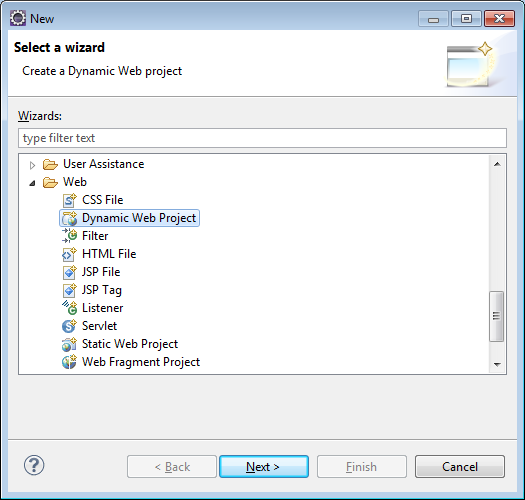
\includegraphics[scale=0.65]{./imagens/apendice_img1.png}}
%   \caption[Exemplo de criação de um projeto Web no Eclipse]
%           {Exemplo de criação de um projeto Web no Eclipse. \textbf{Fonte:} \cite{correa2003plantas}}
% \label{fig:exemplo1}
% \end{figure}
% 
% \par Perceba que o \LaTeX~faz a numeração automática das figuras e já adiciona na lista de figuras.
% 
% \par Agora a mesma imagem foi incluída, porém em escala menhor, conforme ilustra a Figura~\ref{fig:exemplo2}.:
% 
% \begin{figure}[h!]
%   \centerline{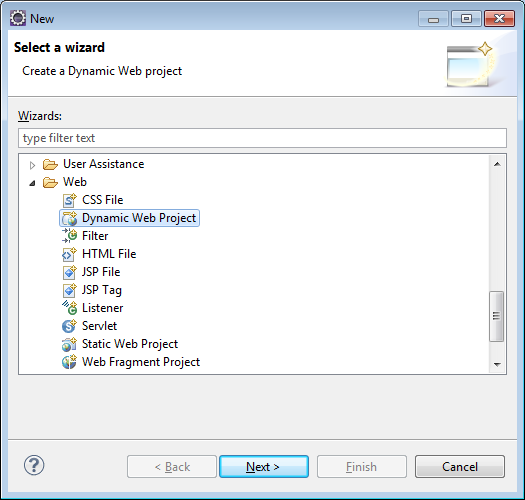
\includegraphics[scale=0.25]{./imagens/apendice_img1.png}}
%   \caption[Mesma imagem em escala menor]
%           {Mesma imagem em escala menor. \textbf{Fonte:} \cite{correa2003plantas}}
% \label{fig:exemplo2}
%\end{figure}


\subsection{PostgreSQL}

\par O PostgreSQL é um banco de dados relacional desenvolvido pela universidade
da California por volta de 1970. Na época o projeto se chamava Ingres e só
passou a se chamar Postgres por volta de 1986 quando Michael Stonebraker adicionou
o conceito de orientação a objetos ao projeto e decidiu então definir um novo
nome para a nova versão.\cite{livro_postgres_doulgas},
\par Para \citeonline{livro_introd_sistemas_bd} , ``um banco de dados é um
sistema computadorizado cuja funcionalidade geral é armazenar informações e
permitir que os usuários busquem e atualizem essas informações quando as
solicitar''. Já o conceito de banco de dados relacional é definido por
\citeonline[p.30]{oracle_database_sql} como:
\begin{citacao}
uma coleção de informações relacionadas, organizadas em tabelas. Cada tabela
armazena dados em linhas; os dados são organizados em colunas. As tabelas são
armazenadas em esquemas de banco de dados, que são áreas  onde os usuários 
podem armazenar suas próprias tabelas.
\end{citacao}
 \par Para manipular e acessar as informações em um banco de dados relacional
 é usado uma linguagem denominada SQL (\textit{Structured Query Language}), que
 foi projetada a especificamente para este fim. A linguagem foi desenvolvida
 pelo IBM por volta de 1970 que tomou como base o trabalho do Dr. E.F.Codd
e possui uma sintaxe simples de fácil aprendizado e utilização.
\cite{oracle_database_sql}


%\par Segundo a Apache (2015), o Tomcat é um software livre que realiza a
%implementação de especificações do Java voltado para programação para 
%internet lançado pela própria Apache.
% \par Exemplo de parágrafo utilizando comando para formatar em itálico as palavras em inglês, como por exemplo: \textit{pets, animals and software} e um exemplo de texto em negrigo: \textbf{grafo}.
% 
% \par Um tipo de citação: segundo \citeonline{correa2003plantas} as plantas \ldots.
% 
% \par Outro tipo de citação: as plantas \ldots \cite{correa2003plantas}.
% 
% \par Outro tipo de citação com página: \cite[p. 13]{correa2003plantas}.
% \par Outro tipo ainda de citação com página:  \citeonline[p. 13]{correa2003plantas}.
% 
% \par Para referenciar seções e capítulos, é necessário colocar o \textbackslash label e a referência assim: na \autoref{sec:materiais} e no \autoref{cap:quadroMetodologico} são encontradas as informações\ldots
% 
% \par Exemplo de equação:
% 
% \begin{equation}
%  \Delta Q = 
%  \left[
%  \frac{\sum_{in} + k_{i,in}}{2m} - 
%  \left(
%  \frac{\sum_{tot} + k_i}{2m}
%  \right)^2
%  \right] -
%  \left[
%  \frac{\sum_{in}}{2m} - 
%  \left(\frac{\sum_{tot}}{2m}
%  \right)^2 - 
%  \left(\frac{k_i}{2m}
%  \right)^2
%  \right]
% \end{equation}
% 
% 
% \par Símbolos matemáticos só funcionam dentro do ambiente \texttt{equation} ou entre dois símbolos \$. Ex: Adiciona cada vértice $w \in N_d(v) \Delta \Gamma$ na região, os quais foram vistos por pelo menos a uma fração $\gamma$ dos vértices em $N_d(v)$.
% 
% \par Outra fórmula: $y=x^2$
% 
% \section{Materiais}
% \label{sec:materiais}
% 
% \par Este parágrafo mostra um exemplo de um teste de nota de rodapé, utilizando o texto do documento da Univas\footnote{O nome “Desenvolvimento” é muito vago, portanto, não o utilize; prefira, de acordo com a situação, ``Fundamentação teórica'', ``Análise dos dados'', ``Objetivos'', ``Metodologia'', etc. }. Outro tipo de nota de rodapé\footnote{\cite{correa2003plantas}}.  Outro tipo ainda de nota de rodapé\footnote{\citeonline{correa2003plantas}}
% 
% 
% \par Um exemplo de tabela é mostrado na Tabela~\ref{tab:informativa}
% 
% 
% \begin{table} [h]
%   \caption[Informação nutricioal dos alimentos]
%           {Informação nutricioal dos alimentos \textbf{Fonte:} \cite{correa2003plantas}}
%   \centering
%   \begin{tabular}{|p{0.7in}|p{2in}|p{3in}|}
%     \hline 
%     \multicolumn{1}{|c|}{\textbf{Hortaliça}} & \multicolumn{1}{c|}{\textbf{Valor Nutricional}} & \multicolumn{1}{c|}{\textbf{Propriedades medicinais}} \\
%     \hline 
% Tomate
% &Vitamina A, C, E e ferro, potássio
% &Maior resistência aos vasos sanguíneos, combate a infecções\\
%     \hline 
% Cenoura
% &Vitamina A, vitaminas do complexo B, cálcio, fósforo
% &Regula o aparelho digestivo, purifica a bile e fortalece a pele\\
%     \hline
% Cebolinha
% &Cálcio, ferro, niacina
% &Estimula o apetite, ajuda na formação de ossos e dentes\\
% 
%     \hline
% Alface
% &Ferro, cálcio, niacina, vita\-mina C
% &Combate insônia, ajuda na cicatrização dos tecidos\\
% 
%     \hline
% Rúcula
% &Iodo, vitaminas A e C
% &Combate a fadiga, depura o sangue\\
% 
%     \hline
% Erva cidreira
% &Sais minerais
% &Tonico nervoso, combate cólicas intestinais\\
% 
%     \hline 
%   \end{tabular}
%   \legend{Fonte: \cite{correa2003plantas}}
%   \label{tab:informativa}
% \end{table}
% 
% \par A seguir segue exemplo de listagem numérica:
% 
% \begin{enumerate}
%   \item conteúdo do item 1;
%   \item conteúdo do item 2;
%   \item conteúdo do item 3;
%   \item conteúdo do item 4;
%   \item conteúdo do item 5;
%   \item conteúdo do item 6;
%   \item etc.
% \end{enumerate}
% 
% \par Também é possível fazer a lista de itens:
% 
% \begin{itemize}
%   \item conteúdo do primeiro item;
%   \item conteúdo do segundo item;
%   \item conteúdo do terceiro item;
%   \item conteúdo do quarto item;
%   \item conteúdo do quinto item;
%   \item etc.
% \end{itemize}
% 
% \par Um exemplo de imagem é mostrado na Figura~\ref{fig:exemplo1}.
% 
% \begin{figure}[h!]
%   \centerline{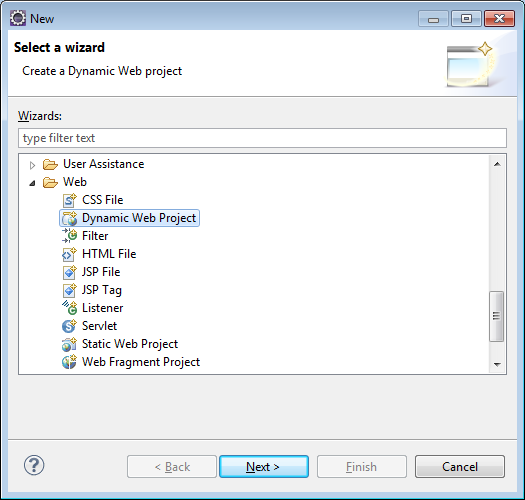
\includegraphics[scale=0.65]{./imagens/apendice_img1.png}}
%   \caption[Exemplo de criação de um projeto Web no Eclipse]
%           {Exemplo de criação de um projeto Web no Eclipse. \textbf{Fonte:} \cite{correa2003plantas}}
% \label{fig:exemplo1}
% \end{figure}
% 
% \par Perceba que o \LaTeX~faz a numeração automática das figuras e já adiciona na lista de figuras.
% 
% \par Agora a mesma imagem foi incluída, porém em escala menhor, conforme ilustra a Figura~\ref{fig:exemplo2}.:
% 
% \begin{figure}[h!]
%   \centerline{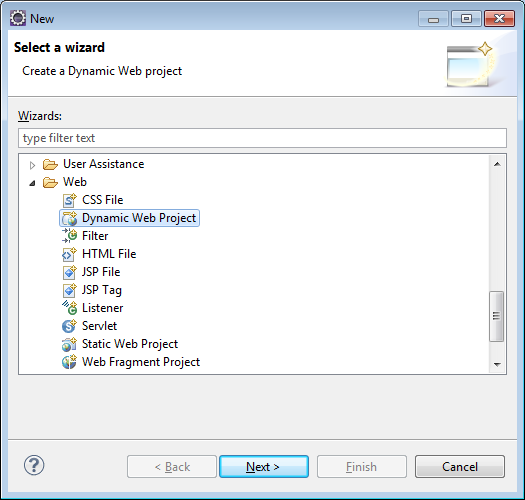
\includegraphics[scale=0.25]{./imagens/apendice_img1.png}}
%   \caption[Mesma imagem em escala menor]
%           {Mesma imagem em escala menor. \textbf{Fonte:} \cite{correa2003plantas}}
% \label{fig:exemplo2}
%\end{figure}



% \par    Desta forma surge a necessidade de primeiramente descrever os
% princípios da teoria proposta por Darwin para que se possa ter um melhor
% entendimento do contexto de computação evolucionária e de algoritmos genéticos.
% É importante, porém, ressaltar que o conteúdo desta sessão não tem como
% objetivo levantar questões sobre o tema da origem dos seres vivos. 
% 	
% \par	O autor afirma ainda que o trabalho de Darwin iniciou-se p
% Esta observação foi o ponto chave que levou o inglês a criar a teoria da evolução. 
% 	
% \par 	Ainda segundo Linden, a teoria afirma que,  

% \par algoritmos genéticos são um ramo de uma das abordagens da inteligência
% artificial denominada abordagem evolutiva. Segundo Lacerda e Carvalho o termo,
% proposto inicialmente por John Holland em 1975 e popularizado através de seu aluno Goldberg
% em 1989, está fundamentado no princípio de seleção natural proposto por Charles Darwin em seu
% livro A Origem das Espécie.
% 
% \par Darwin (1859) propôs que os indivíduos mais fortes evoluem através do processo de
% seleção natural, que define que o indivíduos com melhor capacidade de adaptação ao seu
% ambiente possuem maior chance de sobreviver e gerar descendentes. Algoritmos genéticos
% seguem este mesmo conceito, pois, segundo \citeonline{livro_ags_ricardo_linden},
% são um ramo de um modelo computacional conhecido como algoritmos evolucionários e como tal definem­se como uma
% técnica de otimização e busca que se baseia na teoria do processo de evolução
% natural. \citeonline {livro_ags_ricardo_linden} afirma,
% 
% \begin{citacao}
% “Algoritmos evolucionários funcionam mantendo uma população de estruturas,
% denominadas indivíduos ou cromossomos que se comportam de forma semelhante a
% evolução das espécies. A estas estruturas são aplicados os chamados operadores
% genéticos, como recombinação, mutação, entre outros. Cada indivíduo recebe uma 
% avaliação que é uma quantificaçâo da sua qualidade como solução do problema em
% questão. Com base nesta avaliação serão aplicados os operadores genéticos de forma
% a simular a sobrevivência do mais apto”.\cite[p. 16]{livro_ags_ricardo_linden}
% \end{citacao} 
% 
% \par Técnicas de busca e otimização se destacam pois melhores soluções para um
% problema impacta, muitas vezes, em economia de recursos e neste contexto AGs 
% desempenham um papel importante, pois, como afirma
% \citeonline{nocoes_geriais_anita_fernandes}, “apesar de não garantir que os AGs
% encontrem a solução ótima do problema, existem evidências empíricas de que
% respostas aceitáveis podem ser obtidas em um tempo bastante razoável”.

